\documentclass{article}
\usepackage{graphicx} 
\usepackage[english,ukrainian]{babel}
\usepackage[letterpaper,top=2cm,bottom=2cm,left=3cm,right=3cm,marginparwidth=1.75cm]{geometry}
\usepackage{amsmath, graphicx, booktabs, listings, xcolor, tcolorbox, lipsum, siunitx, multirow, hyperref, pgfplots, inputenc}

\title{Застосування алгоритму index-calculus для дискретного логарифмування}
\date{}

\begin{document}

\maketitle

\section{Мета}
\quad Ознайомлення з алгоритмом дискретного логарифмування index-calculus. Програмна реалiзацiя
цього алгоритму та визначення його переваг, недолiкiв та особливостей застосування. Практична оцiнка
складностi роботи та порiвняння рiзних реалiзацiй цього алгоритму.

\section{Постановка задачі}
\quad Імплементація алгоритму index-calculus

\section{Приклад роботи програми}
\quad 
Testing Index-Calculus with a = 179, b = 97, p = 191 digit length: 3, IC result: x = 168 (took 0.001 seconds)

Testing Index-Calculus with a = 3086, b = 2576, p = 3617 digit length: 4, IC result: x = 1038 (took 0.002 seconds)

Testing Index-Calculus with a = 606, b = 19755, p = 33773 digit length: 5, IC result: x = 9717 (took 0.004 seconds)

Testing Index-Calculus with a = 69366, b = 534740, p = 889081 digit length: 6, IC result: x = 630451 (took 0.014 seconds)

Testing Index-Calculus with a = 3842476, b = 6675652, p = 8043979 digit length: 7, IC result: x = 7268042 (took 0.04 seconds)

Testing Index-Calculus with a = 66830006, b = 51535128, p = 87321277 digit length: 8, IC result: x = 26090344 (took 0.12 seconds)

\section{Замір часу роботи}
\quad На графіку показано залежність часу обчислень від порядку числа.

\begin{figure}[htbp]
    \centering
    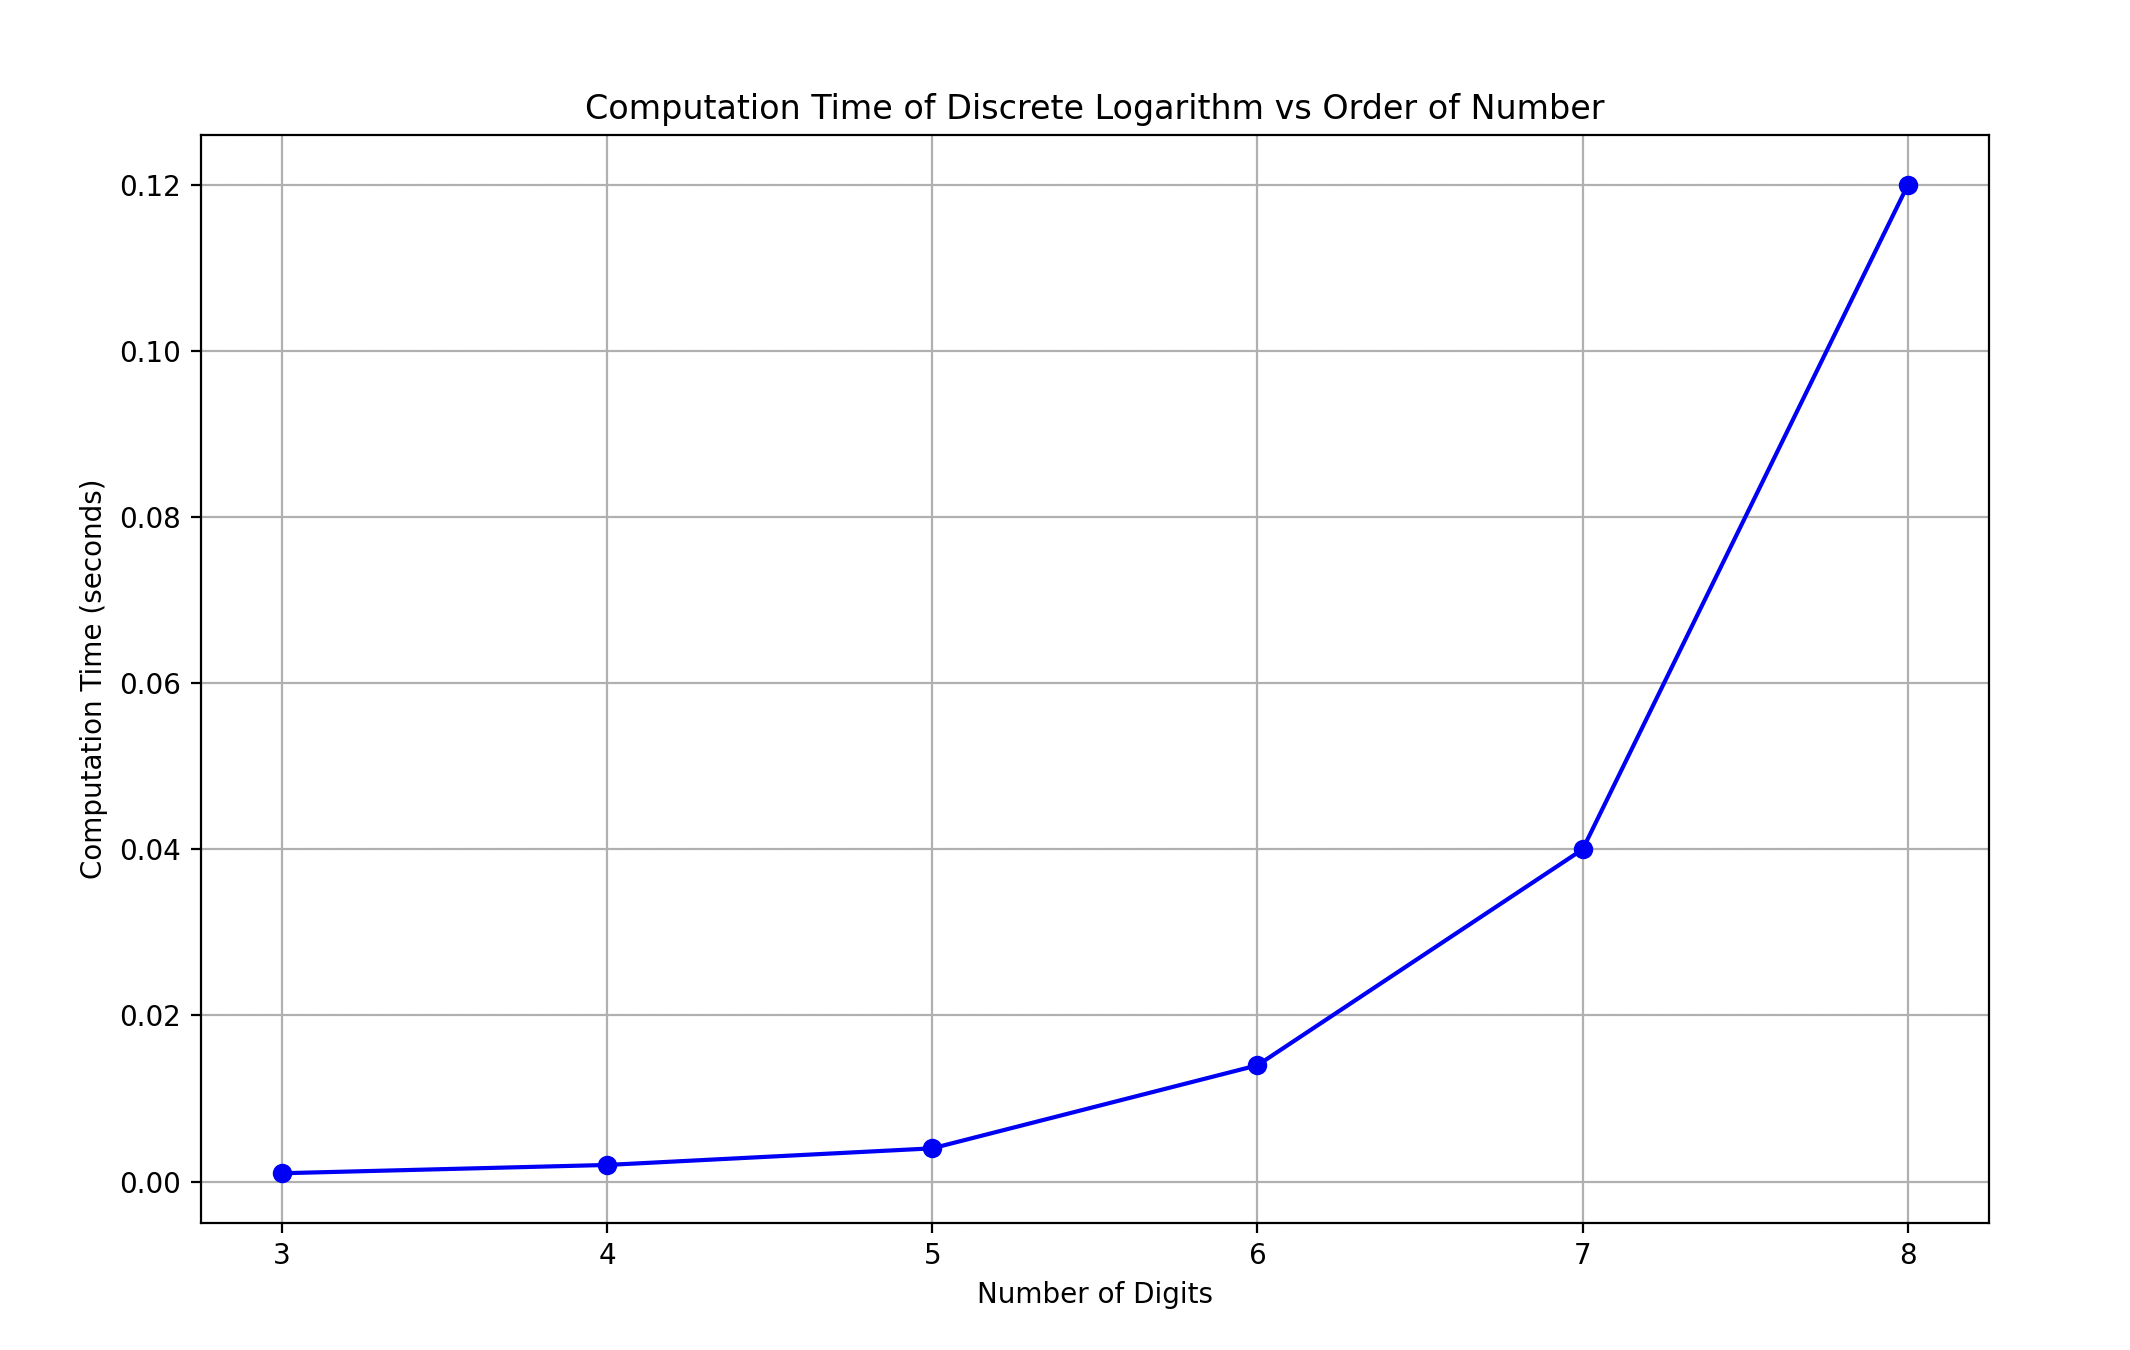
\includegraphics[width=1.0\textwidth]{graphic.png}
    \caption{час роботи}
    \label{fig:screenshot}
\end{figure}

\section{Висновок}
\quad
У цій роботі було розроблено програму для розв'язку задачі дискретного логарифму використовуючи index-calculus, автоматизовано заміри часу роботи розробленого алгоритму.
\end{document}
